\documentclass{report}
\usepackage{amssymb}
\usepackage{amsmath} % Per le formule matematiche
\usepackage{tikz}    % Per i diagrammi

\input{../LatexTemp/preamble}
\input{../LatexTemp/macros}
\input{../LatexTemp/letterfonts}

\newcommand{\dperp}{\mathrel{\bot\!\!\!\bot}} % Independent events

\title{\Huge{Probabilità}\\Appunti}
\author{\huge{Giovanni Palma e Alex Basta}}
\date{}
\pagenumbering{gobble}

\graphicspath{{paginette/img/}}

\begin{document}

\maketitle
\newpage% or \cleardoublepage
% \pdfbookmark[<level>]{<title>}{<dest>}
\pdfbookmark[section]{\contentsname}{toc}




\tableofcontents

\pagebreak
\chapter{Introduzione}

Appunti di Probabilità presi in base alle lezioni di Elly Shlein
% \begin{document}

\chapter{Spazi di probabilità discreti}
\section{Concetti introduttivi}
Innanzi tutto andiamo a definire che cosa intendiamo per \textit{esperimento aleatorio, esito, probabilità}

Con la dicitura esperimento \textit{aleatorio indicheremo} qualunque fenomeno (fisico, economico, sociale, \dots ) il cui esito non sia determinabile con certezza a priori. Il nostro obiettivo è di fornire una descrizione matematica di un esperimento aleatorio, definendo un modello probabilistico, un \textit{esito} invece è un ipotetico risultato di un'esperimento aleatorio sulla base di un cosiddetto \textit{spazio campionario} un insieme che contiene tutti gli esiti possibili dell’esperimento

\esempio{
    \begin{itemize}
        \item \textbf{Esperimento aleatorio:} Lancio di un dado.
        \item \textbf{Spazio campionario:} $\Omega = \{1, 2, 3, 4, 5, 6\}$.
        \item \textbf{Esito:} $4$.
    \end{itemize}
}

\nt{
  In casi piu' complessi ci saranno vari sotto-esperimenti aleatori, come 10 lanci di un dato.
}

Adesso forniamo vere e priorie definizioni
\dfn{evento}{
    Si definisce \textbf{evento} un'affermazione riguardante l'ipotetico esito univoco dell'esperimento, di cui si può affermare con certezza se è vero o falso una volta noto l'esito
}
\ex{}{
    Esper. aleatorio: Lancio del dado\\
    $A = \text{"esce un numero pari"}$
}

\dfn{Spazio camipionario}{
  Si chiama \textit{spazio campionario} un qualunque insieme $ \Omega $ che contiene tutti gli esiti dell'esperimento aleatorio.
}

Notare che non dice "tutti e solo tutti", quindi \textbf{tutti} gli insiemi a cui appartengono gli esiti sono degli spazi campionari.

\ex{Lancio dado}{
  Possiamo porre come spazio campionario:
  \[
  \Omega = \{1,2,3,4,5,6\}
  \]
  ma anche
  \[
  \Omega = \mathbb{R}
  \]
}

\dfn{Esiti favorevoli}{
  Esiti per cui un evento e' vero sono detti esiti favorevoli.
}

\dfn{Evento in termine di insiemi}{
  Un evento si puo' definire anche come il sottoinsieme dello spazio campionario $ \Omega $ formato da tutti gli esiti favorevoli dell'evento.
}

\ex{}{
$ \Omega = \{1,2,3,4,5,6\} \implies A = \text{"esce un numero pari"} = \{2,4,6\} = \text{evento}$
 } 

 \nt{
   La definizione insiemistica di evento dipende dallo spazio campionario definito, mentre l'insieme degli esiti favorevoli e' fisso e rappresenta l'insieme evento di cardinalita' maggiore possibile (esiti favorevoli di $A \subseteq \Omega $).
 }

\dfn{}{
  \begin{itemize}
    \item $ \Omega $ e' l'evento \textit{certo}
    \item $ \emptyset $ e' l'evento \textit{impossibile}
    \item $ \omega \in \Omega $ e' un evento \textit{elementare} ($ A = \{\omega\} $)
  \end{itemize}
}
\ex{}{
  Lancio un dado.
  \[
  A = \text{"esce un numero naturale tra 1 e 6"}
  \]
  \[
  B = \text{"esce un numero maggiore di 6"}
  \]
  \[
  C = \text{"esce il numero 3"}
  \]
  \begin{itemize}
    \item $ \Omega = \{1,2,3,4,5,6\} \implies A = \Omega (evento certo), B = \emptyset (evento impossibile), C = \{3\} $
    \item $ \Omega = \mathbb{R} \implies A = \{1,2,3,4,5,6\} \neq \Omega (evento quasi certo), B = (6,+\infty) (evento quasi impossibile), C = \{3\} $
  \end{itemize}
}

\section{Regole del calcolo probabilistico}
Ad ogni relazione logica possiamo associare un'operazione insiemistica:

\begin{center}
  \begin{tabular}{c|c}
    Connettivi Logici & Connettvi Insiemistici\\
    \hline
    $ A \lor B $ & $ A \cup B $ \\
    $ A \land B $ & $ A \cap B $ \\
    $ \neg A $ & $ A^{c} $ \\
    $ A \implies B $ & $ A \subseteq B $ \\
    $ A \iff B $ & $ A = B $
\end{tabular}
\end{center}

\nt{
  Nella prima colonna, $ A $ e $ B $ sono eventi come affermazioni, mentre nella colonna di destra sono degli insiemi.
}


\subsection{Assiomi della probabilita'}
Poniamo tre assimi fondamentali da cui possiamo partire per derivare tutte le operazioni e proprieta' che ci servono:

\nt{
  Per noi tutti i sottoinsiemi di $ \Omega $ sono eventi (anche se non sara' sempre cosi)
}
\dfn{Assioma 1}{
  A ciascun sottoinsieme $ A $ di $ \Omega $ ($ \forall A \in \powerset(\Omega) $) e' assegnato un numero che chiamo $ \mathbb{P}(A) \in [0,1] $. Questo numero si chiama \textit{probabilita'} di $ A $.
}

\nt{
  Quindi, per il primo assioma, esiste una funzione probabilita' $ \mathbb{P}(A): \powerset (\Omega) \to [0,1] $.
}

\dfn{Assioma 2}{
  Dato $ \Omega $ spazio campionario:
  \[
   \mathbb{P}(\Omega) = 1 
  \]
}

\dfn{Assioma 3: Proprieta' di sigma addittivita'}{
  Sia $ (A_n)_{n \in \mathbb{N}} $ una sequenza di insiemi (eventi) tali che $\forall i \neq j. A_i \cap A_j = \emptyset  $ (insiemi disgiunti) si ha che:
  \[
  \mathbb{P}\left(\bigcup_{i=1}^{\infty}  A_i\right) = \sum_{i=1}^{+\infty}\mathbb{P}(A_i)
  \]
  Quindi la probabilita' di un unione infinita di eventi \textbf{disgiunti} e' uguale alla somma delle probabilita' dei singoli eventi.
}


\dfn{Probabilita' discreta}{
  Chiamo probabilita' discreta una funzione probabilita' $ \mathbb{P} $ a valori discreti, ovvero che puo' assumere un numero finito o al piu' numerabile di valori fra 0 e 1.
}

Vediamo una tale probabilita':

\dfn{Delta di Dirac}{
  Sia $ \Omega = \mathbb{R}, x_0 \in \mathbb{R} $, allora si chiama delta di Dirac centrato in $ x_0 $ la funzione:
\[
  \begin{aligned} 
    \delta_{x_0}: \powerset(\mathbb{R}) &\to [0,1]\\
    A &\mapsto \delta_{x_0}(A) = \begin{cases}
    1 & x_0 \in A\\
    0 & x_0 \notin A
    \end{cases}
  \end{aligned}
\]
}

Notare che per definizione, la funzione di Dirac e' una probabilita' discreta, dato che soddisfa tutti gli assiomi (ma non molto utile dato che assume solo due valori). Pero', tramite le delta di Dirac siamo in grado di costruire qualunque altra probabilita' discreta:

Sia $ \Omega = \mathbb{R}$. Prendiamo un numero contabile $ n $ di eventi singoletto $ x_1,x_2,...,x_n \in \mathbb{R} $ a cui corrispondono $ p_1,p_2,...,p_n \in \mathbb{R} $ tale che:
\[
 \forall i = 1,...,n.\ p_i \in [0,1], \qquad  \sum_{i=1}^{n} p_i = 1 
\]
Definiamo la funzione:
\[
\begin{aligned}
  \mathbb{P}: \powerset(\Omega) &\to [0,1]\\
  A &\mapsto \sum_{i=1}^{n} p_i \delta_{x_i}(A)
\end{aligned}
\]
$ \mathbb{P} $ e' una combinazione lineare di delta di Dirac. Essendo una combinazione convessa, $ \mathbb{P} \in [0,1] $ e si puo' dimostrare che soddisfa gli altri due assiomi, quindi e' una probabilita' discreta! Variando le $ x $ e le $ p $ e' possibile generare qualsiasi funzione $ \mathbb{P} $ discreta.

\ex{}{
  $ \Omega = \{1,2,3,4,5,6\},\ \forall i = 1,...,6.\ x_i = i,\ p_i = \frac{1}{6} $, la funzione $ \mathbb{P} $ associata e':
  \[
   P(A) = \sum_{ i=1}^{6} \frac{1}{6} d_{x_i}(A)
  \]
  \[
    A = \{1,2,3,4,5,6\} \implies P(A) = 1 
  \]
  \[
    B = (6,+\infty) \implies P(B) = 0
  \]
  \[
    C = \{1,2,3,4,5,6,7,8,9\} \implies P(C) = 1
  \]
}

\dfn{}{
  Si chiama evento quasi certo un evento $ A.\ P(A) = 1 $
}

\dfn{}{
  Si chiama evento quasi impossibile un evento $ A.\ P(A) = 0 $
}

Posso allargare $ \Omega $ quanto voglio perche' tanto fuori dall'insieme minimo che comprende tutti gli eventi possibili le probabilita' che aggiugo sono quasi impossibili e quindi hanno probabilita' 0 e non cambiano il valore totale della somma.

\subsection{Conseguenze degli assiomi}

\thm{}{
  Sia $ \Omega $ spazio campionario e $ \mathbb{P} $ probabilita' su $ \Omega $ ($ (\Omega, \mathbb{P}) $ e' uno spazio di probabilita' con $ \mathbb{P}: \powerset(A) \to [0,1] $). Dagli assiomi 1,2,3 deduciamo le cose seguenti:
  \begin{enumerate}
  \item $ \mathbb{P}(\emptyset) = 0 $
  \item \textbf{Addittivita' finita}: $ (A_i)_{i = 1,...,n}.\ \forall i \neq j.A_i \cap A_j = \emptyset \implies \mathbb{P}(\bigcup_{i=1}^{n} A_i) = \sum_{i=1}^{n} \mathbb{P}(A_i) $
  \item $\mathbb{P}(A^c) = 1 - \mathbb{P}(A)$
  \item \textbf{Monotonia}: $ A \subseteq B \implies \mathbb{P}(A) \leq \mathbb{P}(B) $
  \end{enumerate}
}

\pf{Dimostriamo}{
  \begin{enumerate}
    \item Devo mostrare che $ \mathbb{P}(\emptyset) = 0$. Per semplicita' definiamo $ p \coloneq \mathbb{P}(\emptyset) $ Uso l'assioma 3 con la successione $ (A_n)_{n \in \mathbb{N}}.\ \forall i \in \mathbb{N}. A_i = \emptyset $, che sono tutti eventi disgiunti, quindi $ \mathbb{P}(\bigcup_{i=1}^{\infty} A_i) = \sum_{i=1}^{\infty} P(A_i) = \sum_{i=1}^{\infty} p $. Inoltre:

\[
\bigcup_{i=1}^{\infty} A_i = \emptyset
\]

Quindi:
\[
p = \sum_{i=1}^{\infty} p = \begin{cases}
0 & p=0\\
  +\infty & p \in (0,1]
\end{cases}
\]
L'equazione e' soddisfatta solo per $ p = 0 $.

\item Suppongo di avere una sequenza finita disgiunta $ A_n $, devo dimostrare che $ \mathbb{P}(\bigcup_{i=1}^{n} A_i) = \sum_{i=1}^{n} \mathbb{P}(A_i) $. Definisco $ (B_i)_{i \in \mathbb{N}} $ tale che $ B_i = A_i \forall i = 1,...,n $ e $ \forall i > n. B_i = \emptyset $. Usando l'assioma 3:
  \[
    \mathbb{P}\left(\bigcup_{i=1}^{\infty} B_i\right) = \sum_{i=1}^{\infty} \mathbb{P}(B_i) = \sum_{i=1}^{n} A_i 
  \]
\item Devo dimostrare che $ \mathbb{P}(A^{c}) = 1 - \mathbb{P}(A) $. Per definizione di complemento $ A^{c} + A = \Omega $ e i due insiemi sono disgiunti. Per l'addittivita' $ \mathbb{P}(A^{c}) + \mathbb{P}(A) = \mathbb{P}(A^{c}+A) = \mathbb{P}(\Omega) = 1 $ per l'assioma 2.
\item Assumiamo che $ A \subseteq B $. Dimostriamo che $ \mathbb{P}(A) \leq \mathbb{P}(B) $. Per ipotesi $ B = A \cup (B\setminus A) $, quindi per addittivita' $ \mathbb{P}(B) = \mathbb{P}(A) + \mathbb{P}(B\setminus A) $. Per assioma 1 ovvio.
  \end{enumerate}
}

\thm{Probabilita' unione non disgiunta}{
  siano $ A $ e $ B $ eventi:
  \[
    \mathbb{P}(A \cup B) = \mathbb{P}(A) + \mathbb{P}(B) - \mathbb{P}(A \cap B)
  \]
}

\pf{}{
  $ A \cup B = (A \setminus B) \cup (B\setminus A) \cup (B \cap A) $, quindi per addittivita':
  \[
    \mathbb{P}(A \cup B) = \mathbb{P}(A \setminus B) + \mathbb{P}(B \setminus A) + \mathbb{P}(A \cap B)
  \]
  $ \mathbb{P}(A \setminus B) + \mathbb{P}(A \cap B) = \mathbb{P}(A) $ e $ \mathbb{P}(B \setminus A) + \mathbb{P}(A \cap B) = \mathbb{P}(B)  $ dato che $ (X \setminus Y) \cup (X \cap Y) $, ovvio.
}

\nt{
  La formula si complica con un numero di eventi maggiore di 2, infatti per $ n=3 $:
  \[
    \mathbb{P}(A \cup B \cup C) = \mathbb{P}(A) + \mathbb{P}(b) + \mathbb{P}(C) - \mathbb{P}(A \cap B) - \mathbb{P}(B \cap C) - \mathbb{P}(A \cap C) + \mathbb{P}(A \cap B \cap C)
  \]
}

Provare esercizi (da soli!)

% \end{document}

% \begin{document}
\chapter{Probabilita' Condizionata}

Cosa significa a livello di calcolo conoscere un nuovo evento?

Notazione:
\begin{itemize}
  \item $ \mathbb{P}(A|B) $: probabilita' dell'evento $ A $ condizionata a $ B $
\end{itemize}

Domanda: se so che si e' verificato $ B $, come cambia $ \mathbb{P}(A) $?

\nt{
  $ \mathbb{P}(A|B) = \mathbb{P}(\cdot | B), B \subseteq \Omega $, quindi essendo sempre una probabilita' ha sempre tutte le proprieta' di una qualunque probabilita'. La probabilita' e' sempre relativa ad $ A $, la $ B $ cambia solo come agisce $ \mathbb{P} $
}

\ex{Probabilita' uniforme}{
  Lancio del dado: $ \Omega = \{1,2,3,4,5,6\} $, $ \mathbb{P} $ prop. uniforme

  $ \mathbb{P}(\{\omega\}) = \frac{1}{|\Omega|}, \forall \omega \in \Omega $, ovvero:
  \[
    \mathbb{P}(A) = \frac{\text{casi favorevoli in }A}{\text{casi possibili}}
  \]
  $ A = \text{"esce un numero maggiore di 3"} = \{3,4,5,6\} $ e $ B = \{\text{"esce un numero pari"}\} = \{2,4,6\} $, domanda $ \mathbb{P}(A|B) $?

  $ P(A) = \frac{4}{6} $ come abbiamo gia visto.

  Ora facciamo che sappiamo che $ B $ si sia avverato. ATTENZIONE! cio' non vuol dire che cambia lo spazio campionario perche' l'esperimento e' lo stesso, ma cambiano i \textit{veri} casi favorevoli e i \textit{veri} casi possibili:
  \[
    P(A|B) = \frac{\text{"veri casi favorevoli di A"}}{\text{veri casi possibili}} = \frac{|A \cap B|}{|B|} = \frac{2}{3}
  \]

  Dado a 4 facce truccato: 

  \[
    \mathbb{P}(A|B) = \frac{\text{"probabilita' dei veri casi favorevoli di A"}}{\text{probabilita' dei veri casi possibili}} = \frac{}{}
  \]
}

\dfn{Probabilita' Condizionata}{
  Prendo due eventi $ A, B $, uno spazio di probabilita' $ \left( \Omega, \mathbb{P} \right) $ con 
  \[
    \mathbb{P}(B) > 0
  \]
  Definisco \textit{probabilita' condizionata a B di A} la funzione:
  \[
    \mathbb{P}(A|B) = \frac{\mathbb{P}(A \cap B)}{\mathbb{P}(B)}
  \]
}

\nt{
  Se $ \mathbb{P} $ e' la probabilita' uniforme allora:
  \[
    \mathbb{P}(A|B) = \frac{\mathbb{P}(A \cap B)}{\mathbb{P}(B)} = \frac{\frac{|A \cap B|}{|\Omega|}}{\frac{|B|}{|\Omega|}} = \frac{|A \cap B|}{|B|}
  \]
}

\nt{
  B e' fissato nella definizione di propbabilita' condizionata, ovvero:
  \[
    \mathbb{P}(A|B) \neq \mathbb{P}(B|A)
  \]
  Quindi il ruolo di $ A $ e $ B $ e' completamente diverso
}

\nt{
  Se $ B = \Omega $, allora $ \mathbb{P}(A|B) = \mathbb{P}(A) $ dato che la conoscenza del fatto che si e' avverato $ \Omega $ e' ovvio e non ci cambia.

  Se $ A = \Omega $, allora $ \mathbb{P}(\Omega | B) = 1 $ (per proprieta', dato che e' sempre una probabilita')
}

Verifichiamo gli assiomi (fissiamo $ B \subseteq \Omega $ con $ \mathbb{P}(B) > 0 $):

\begin{enumerate}
  \item $ \mathbb{P}(A|B) \in [0,1], \forall A \subseteq \Omega $
  \item $ \mathbb{P}(\Omega|B) = 1 $
  \item $ \sigma-\text{addittivita'} $: $ (A_i)_{i \in \mathbb{N}} $ disgiunti:
    \[
      \mathbb{P}(\bigcup_{i=1}^{\infty} A_i|B) = \sum_{i=1}^{\infty} \mathbb{P}(A_i|B)
    \]
\end{enumerate}

\nt{
  La probabilita' condizionata in genere e' nota e si usa per calcolare la probabilita' dell'intersezione:
  \[
    \mathbb{P}(A \cap B) = \mathbb{P}(A|B) \cdot \mathbb{P}(B)
  \]
  Questa formula e' detta regola della catena. Vale in generalecon $ n $ eventi
}

\mprop{}{
  $ (A_i)_{i = 1,...,n}, \mathbb{P}(A_1 \cap ... \cap A_{n-1}) > 0 $, allora:
  \[
    \mathbb{P}(A_1 \cap ... \cap A_n) = \mathbb{P}(A_1)\mathbb{P}(A_2|A_1)\mathbb{P}(A_3|A_1 \cap A_2) ... \mathbb{P}(A_n| A_1 \cap ... A_{n-1})
  \]
  La condizione funziona grazie alla monotonia, dato che $ 0 < \mathbb{P}(A_1 \cap ... \cap A_{n-1}) \leq \mathbb{P}(A_1 \cap ... \cap A_j), 1 \leq j \leq n-1 $
}

\section{Eventi indipendenti}
Si osservi la seguente definizione
\dfn{Eventi indipendenti}{
  Due eventi $ A, B $ si dicono indipendenti se:
  \begin{equation}
    \mathbb{P}(A \cap B) = \mathbb{P}(A) \cdot \mathbb{P}(B)
  \end{equation}
  

  E viene denatato $A \dperp B$
}

Generalizzando: 
\dfn{Eventi indipendenti generale}{
  Sia dati $n$ eventi $A_1, A_2, ..., A_n$, essi si dicono indipendenti se:
  \[
    \mathbb{P}(A_1 \cap ... \cap A_n) = \mathbb{P}(A_1) \cdot ... \cdot \mathbb{P}(A_n)
  \]
  
}

L'indipendenza tra due eventi e' una relazione simmetrica, ovvero:
\[
  A \dperp B \iff B \dperp A
\]

In particolare si noti il seguente teorema:
\thm{Teorema della simmetria tra eventi indipendenti}{ \label{thm:simmetria_indipendenza}
  Sia $\mathbb{P}(B)>0$ allora:
  \[
    A \dperp B \iff \mathbb{P}(A|B) = \mathbb{P}(A)
  \]
  Dall'altro lato, sia $\mathbb{P}(A)>0$ allora:
  \[
    A \dperp B \iff \mathbb{P}(B|A) = \mathbb{P}(B)
  \]
}

\pf{Dimostrazione}{
  Verrà fornita solo la dimostrazione del primo punto, la seconda parte è analoga.

  Assumo $\mathbb{P}(B)>0$, si ha:
  \begin{itemize}
    \item $ A \dperp B \implies \mathbb{P}(A|B) = \mathbb{P}(A) $:
      \[
        \mathbb{P}(A|B) = \frac{\mathbb{P}(A \cap B)}{\mathbb{P}(B)} = \frac{\mathbb{P}(A) \cdot \mathbb{P}(B)}{\mathbb{P}(B)} = \mathbb{P}(A)
      \]
    \item $ \mathbb{P}(A|B) = \mathbb{P}(A) \implies A \dperp B $:
      \[
        \mathbb{P}(A \cap B) = \mathbb{P}(A|B) \cdot \mathbb{P}(B) = \mathbb{P}(A) \cdot \mathbb{P}(B)
      \]
  \end{itemize}
}

\nt{
  Si noti che se $\mathbb{P}(A)>0$ e $\mathbb{P}(B)>0$ allora, le tre uguaglianze seguenti sono equivalenti:
  \[
    \mathbb{P}(A\cap B) = \mathbb{P}(A) \cdot \mathbb{P}(B) \iff \mathbb{P}(A|B) = \mathbb{P}(A) \iff \mathbb{P}(B|A) = \mathbb{P}(B)
  \]
}

Adesso fornirò un altro teorema piuttosto importante:
\mprop{Sull'indipendenza di eventi complomentari}{
  Siano $A, B$ due eventi indipendenti, allora:
  \[
    A \dperp B \iff A^c  \dperp B,\, A \dperp B^c,\, A^c \dperp B^c
  \]
}
\pf{Dimostrazione}{
  Dimostro solo la prima parte, le altre sono analoghe.

  Assumo $A, B$ due eventi indipendenti, debbo dimostrare la seguente uguaglianza:
  \[
    \mathbb{P}(A^c \cap B) = \mathbb{P}(A^c) \cdot \mathbb{P}(B)
  \]

  Dato che 
  \[
    B = \Omega \cap B = (A \cup A^c) \cap B = (A \cap B) \cup (A^c \cap B)
  \]

  E dato che $ (A \cap B) $e$ (A^c \cap B)$ sono disgiunti, per \ref{item:finite_additivity} (\textit{additività finita}) si ha:
  \[
    \mathbb{P}(B) = \mathbb{P}(A \cap B) + \mathbb{P}(A^c \cap B)
  \]

  E dato che $ A \dperp B $ si ha:
  \[
    \mathbb{P}(B) = \mathbb{P}(A \cap B) + \mathbb{P}(A^c \cap B) = \mathbb{P}(A \cap B) = \mathbb{P}(A) \cdot \mathbb{P}(B) + \mathbb{P}(A^c \cap B)
  \]
  Quindi:
  \[
    \mathbb{P}(A^c \cap B) = \mathbb{P}(B) - \mathbb{P}(A \cap B) = \mathbb{P}(B) - \mathbb{P}(A) \cdot \mathbb{P}(B) = \mathbb{P}(B) \cdot (1 - \mathbb{P}(A)) = \mathbb{P}(A^c) \cdot \mathbb{P}(B)
  \]
}

\ex{Calcolo di eventi indipendenti con probabilita condizionata}{

\textbf{TESTO:}

    Si lancia un dado a 6 facce

    \( A = \) "Esce un numero \( > 4 \)" \\
    \( B = \) "Esce un numero pari"

    Determinare \( P(A) \) e \( P(A|B) \)

\textbf{DETTAGLIO SVOLGIMENTO:}

    \begin{align*}
        \Omega &= \{1, 2, 3, 4, 5, 6\} \\
        A &= \{ 5, 6\} \\
        B &= \{2, 4, 6\} \\
        P(A) &= \frac{3}{6} = \frac{1}{3} \\
        P(A|B) &= \frac{P(A \cap B)}{P(B)} = \frac{\frac{1}{6}}{\frac{3}{6}} = \frac{1}{3}
    \end{align*}

    Dato che \( P(A) = P(A|B) \), per il teorema \ref{thm:simmetria_indipendenza} si ha che \( A \dperp B \)
}

Ecco un altro eserzio:
\ex{}{
  \textbf{TESTO}

Lanciamo una moneta e un dado a 4 facce.

Determinare uno spazio di prob. che descriva l'esperimento aleatorio

\textbf{SOLUZIONE}

\Omega = \left\{ (T,1), (T,2), (T,3), (T,4), (C,1), (C,2), (C,3), (C,4) \right\}

P(T,1) = \frac{1}{8} = P(C,4) = \frac{1}{8}

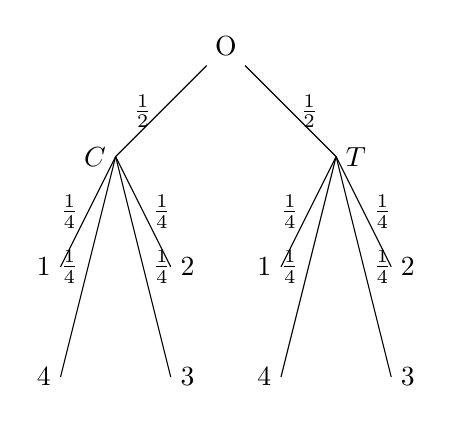
\begin{tikzpicture}[scale=0.7]
    \node (root) at (0,0) {O};
    \draw (root) -- (-2,-2) node[left] {$C$} node[midway,left] {$\frac{1}{2}$};
    \draw (root) -- (2,-2) node[right] {$T$} node[midway,right] {$\frac{1}{2}$};
    
    \draw (-2,-2) -- (-3,-4) node[left] {$1$} node[midway,left] {$\frac{1}{4}$};
    \draw (-2,-2) -- (-1,-4) node[right] {$2$} node[midway,right] {$\frac{1}{4}$};
    \draw (-2,-2) -- (-1,-6) node[right] {$3$} node[midway,right] {$\frac{1}{4}$};
    \draw (-2,-2) -- (-3,-6) node[left] {$4$} node[midway,left] {$\frac{1}{4}$};
    
    \draw (2,-2) -- (1,-4) node[left] {$1$} node[midway,left] {$\frac{1}{4}$};
    \draw (2,-2) -- (3,-4) node[right] {$2$} node[midway,right] {$\frac{1}{4}$};
    \draw (2,-2) -- (3,-6) node[right] {$3$} node[midway,right] {$\frac{1}{4}$};
    \draw (2,-2) -- (1,-6) node[left] {$4$} node[midway,left] {$\frac{1}{4}$};
\end{tikzpicture}

  \[
  \begin{aligned}
  & T = \text{"esito del lancio moneta e testa"} \\
  & C = \text{"esito del lancio moneta è croce"} \\
  & D_i = \text{"è uscito il numero } i \text{"} \\
  & P(C) = \frac{1}{2}, \quad P(T) = \frac{1}{2} \\
  & P(D_i | C) = \frac{1}{4} \\
  & P(D_i | T) = \frac{1}{4} \\
  & A = \text{"è uscito testa e il numero } i \text{"} \\
  & P(A) = P(T) \cdot P(D_i | T) = \frac{1}{2} \cdot \frac{1}{4} = \frac{1}{8} \\
  & \text{Analogamente per } C \cap D_i
  \end{aligned}
  \]
}



% \end{document}


\end{document}
